% 微信服务号介绍页面
\begin{wrapfigure}{L}{5.6cm}
	
\includegraphics[scale=0.7]{picture/scanWechat.jpg}
	\label{fig:scanWechat}
\end{wrapfigure}
微信服务号是对企业版产品的补充,可以让用户在不方便访问企业版WEB和在没有安装企业版APP时可以查询其持有的资产和交易记录(显示最近10条),您可以扫描\hyperref[fig:scanWechat]{\emp{左边二维码}}关注服务号,登录关联企业账号后就可以查看关联账户的资产和交易记录。\par

微信服务号提供了一些基本的功能,主要包括账户绑定微信、切换绑定账户、查看当前绑定的账户信息、查看企业信息、查看企业持有资产、查看交易记录、查看现金宝产品、查看高收益产品、以及可以通过微信服务号申请预约码。\par

\begin{wrapfigure}{R}{0pt}
	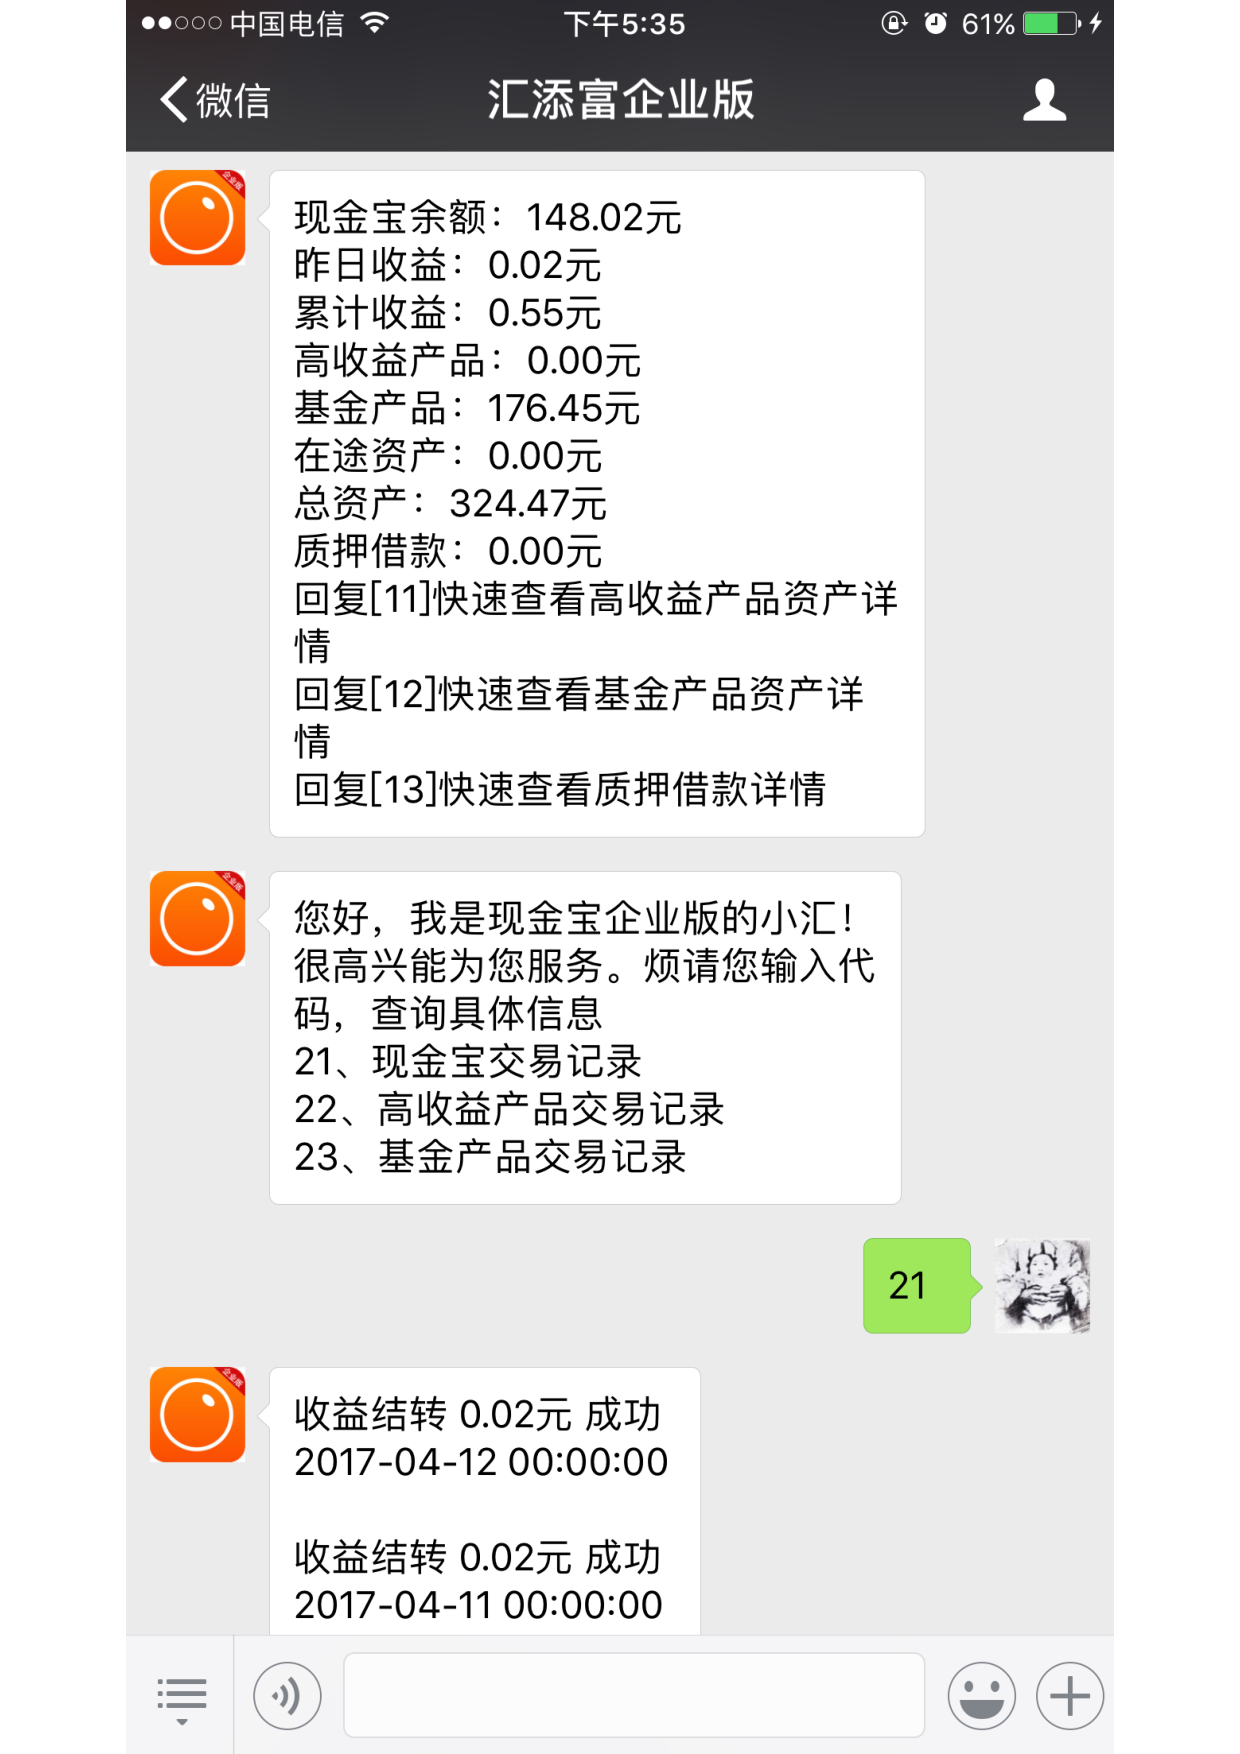
\includegraphics[width=0.45\textwidth]{picture/weixin.pdf}
	\label{fig:weixin}
\end{wrapfigure}

基于微信的方便性和易用性,随时可以获取企业的重要数据,给用户带来了便利性。另外,微信服务号基于微信平台,具有跨平台的功能。\par

出于安全性考虑,以及企业版的交易功能比较复杂,且具有非常规的流程,所以交易功能不予提供。\par

后续为了更方便的服务用户,经办员发起业务的消息会通过微信服务号推送至复核员,并且提供H5页面以方便复核员查看并复核业务。\par

另外,微信服务号可以通过H5页面的方式访问并查看现金宝、高端理财和基金的产品。

